\documentclass[12pt]{article}
\usepackage{amsmath}
\usepackage{amssymb}
\usepackage{amsthm}
\usepackage{amsfonts}
\usepackage{algpseudocode}
\usepackage{algorithm}
\usepackage{mathrsfs}
\usepackage{graphicx}
\usepackage{times}
\usepackage{color}
\usepackage{appendix}
\usepackage{subfigure}
\usepackage{enumerate}
\usepackage{mathtools}
\usepackage{multirow}
\usepackage{booktabs}
\numberwithin{table}{section}
\usepackage{enumitem} %change list depth
\usepackage{hyperref}
\usepackage{listings}
\usepackage{xcolor}

\definecolor{codegreen}{rgb}{0,0.6,0}
\definecolor{codegray}{rgb}{0.5,0.5,0.5}
\definecolor{codepurple}{rgb}{0.58,0,0.82}
\definecolor{backcolour}{rgb}{0.95,0.95,0.92}

\lstdefinestyle{mystyle}{
	backgroundcolor=\color{backcolour},   
	commentstyle=\color{codegreen},
	keywordstyle=\color{magenta},
	numberstyle=\tiny\color{codegray},
	stringstyle=\color{codepurple},
	basicstyle=\ttfamily\footnotesize,
	breakatwhitespace=false,         
	breaklines=true,                 
	captionpos=b,                    
	keepspaces=true,                 
	numbers=left,                    
	numbersep=5pt,                  
	showspaces=false,                
	showstringspaces=false,
	showtabs=false,                  
	tabsize=2
}

\lstset{style=mystyle}

\usepackage{tikz}
\usetikzlibrary{positioning}
\usetikzlibrary{arrows,arrows.meta}
\setlistdepth{8}
\renewlist{itemize}{itemize}{8}

\newcommand{\question}[2][]{\begin{flushleft}
		\Large\textbf{Question #1}: \large\textit{#2}
		
\end{flushleft}}
\newcommand{\sol}{\textbf{Solution}:} %Use if you want a boldface solution line
\newcommand{\maketitletwo}[2][]{\begin{center}
		\Large{\textbf{Homework #1}
			
			ECE 590: Towards More Reliable Software} % Name of course here
		\vspace{5pt}
		
		\normalsize{Jeff Fan  \hspace{1em} $\left|\right|$ \hspace{1em}zf70@duke.edu  % Your name here
			
			\today}        % Change to due date if preferred
		\vspace{15pt}
		
\end{center}}

\begin{document}
	\maketitletwo[8]  % Optional argument is assignment number
	%Keep a blank space between maketitletwo and \question[1]
	
	\section*{Question 1: } 
	\textbf{a.}
	
	The code continuously creates new processes in an infinite while loop without any break condition or pause. This can lead to an AR-fault because it will repeatedly call fork() without limit, potentially exhausting system resources by creating an excessive number of processes.\\
	\\
	\textbf{b.}
	
	The error caused by activating the AR-fault would be that the system runs out of process IDs or memory to allocate for new processes. Each new process requires a certain amount of resources, and systems have a maximum number of concurrent processes they can handle. When this limit is reached, no new processes can be created, which could cause system instability or even a crash. Additionally, if system resources are exhausted, other users and processes will be unable to perform tasks normally, leading to a denial of service.\\
	\\
	\textbf{c.}
	
	The aging effects caused by the causality chain composed of (a) and (b) could mean that as the system continues to run this code, it will increasingly consume more resources, leaving less available for other processes. Over time, the performance of the system may degrade as the process table becomes filled with child processes that are created but never terminated (since there is no wait system call to clean up the child processes). This may lead to longer process creation times, slower system response, and eventually a complete inability to create new processes. This is especially problematic for systems that are expected to run continuously over long periods, as the accumulation of unused resources can lead to a system halt or crash.
	
	\section*{Question 2: } 
	\textbf{a.}
	It is non-linear.
	
	The accumulation rate is represented by the differences in memory sizes from one month to the next, and we can calculate the rate of change of this accumulation rate to see if it increases, decreases, or remains constant as memory size increases.
	
	\begin{center}
		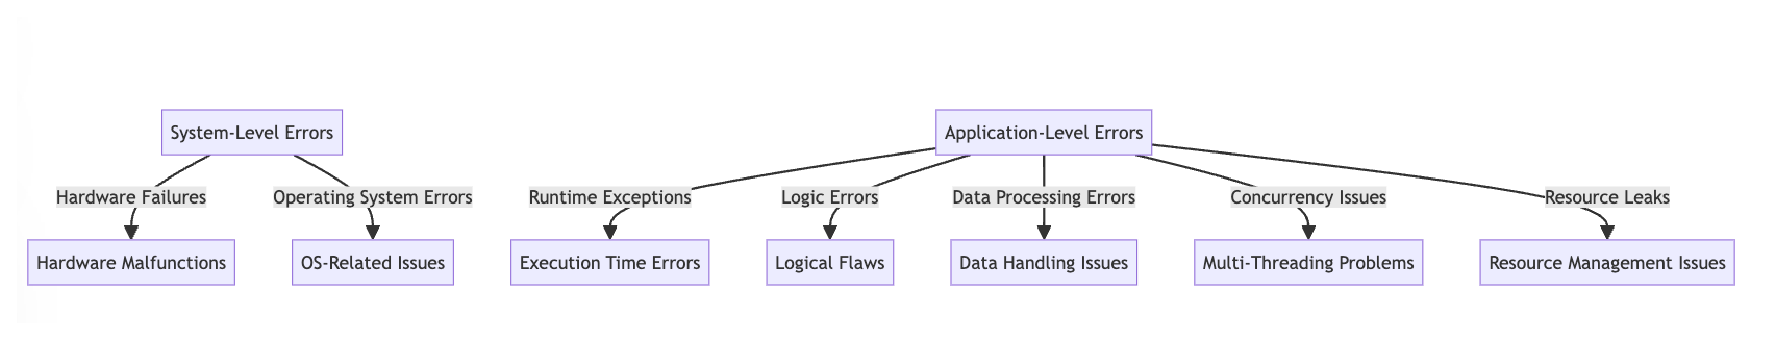
\includegraphics[width=1\textwidth]{image/1.eps}
	\end{center}

	The aging effect accumulation rate depicted in the graph is non-linear. This can be justified by observing the rate of change between consecutive months. In a linear relationship, we would expect to see a constant rate of change, meaning that the percentage increase or decrease between each month would be the same.
	
	However, in this graph, the percentage change is highest between the second and third months (486\% to 160.41\%) and then decreases progressively with each subsequent month. The rate of decrease slows down as time progresses, which is indicative of a decelerating growth rate, a characteristic of non-linear behavior.

	This type of decay is often seen in natural processes where the effect is strongest at the beginning and then diminishes over time, following a logarithmic or exponential decay model rather than a linear model.
	
	\begin{center}
		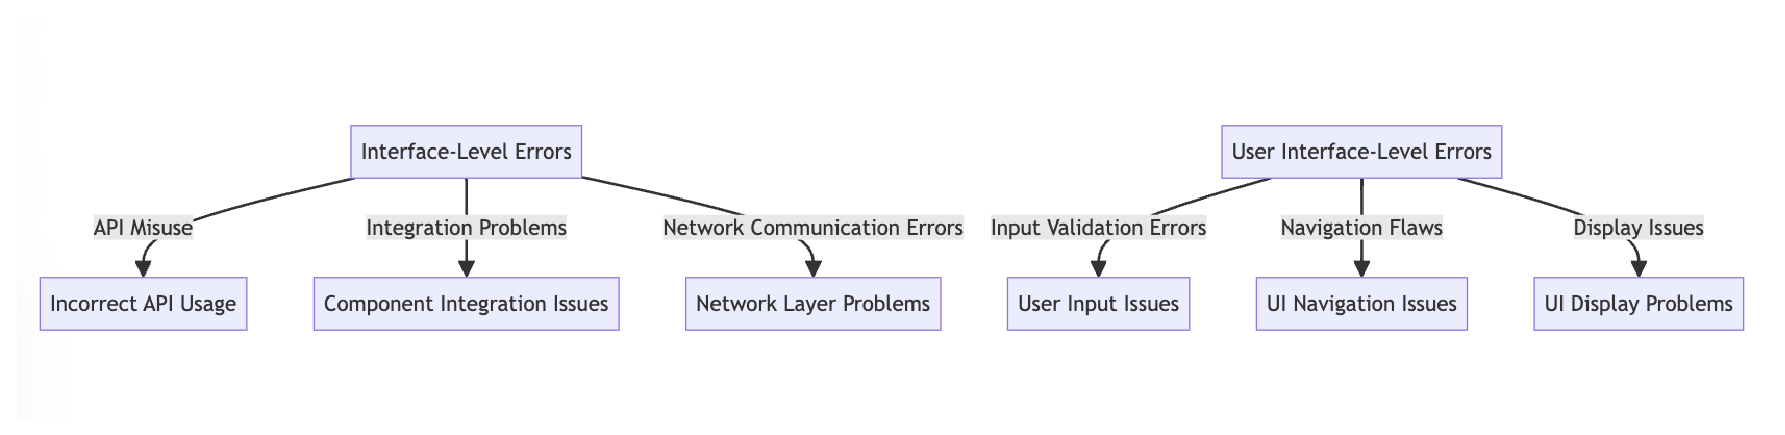
\includegraphics[width=1\textwidth]{image/2.eps}
	\end{center}
	
	The data has been fitted to both an exponential decay model and a logarithmic decay model. The parameters for the exponential decay model are approximately $a= 4950.88643,  b=1.16723363, and 
	c=7.00813855. $ The exponential model seems to have converged. Above is the graph with the original data points and the fitted exponential decay curve. The exponential decay model is displayed in red.
	
	The red curve represents the exponential decay fit to the data points. The parameters for this model indicate the initial value  $a$, the decay rate $b$, and the horizontal asymptote $c$ to which the model approaches as $x$ increases.\\
	\\
	\textbf{b.}
	
	It is about 21 months.
	
	In the same way, the analysis of the memory size growth using a logarithmic decay model suggests that the expected time to AR-failure, or the point at which the process will exceed the critical limit of 2.8 gigabytes and be terminated by the satellite operating system, is approximately 21 months from the start of the monitoring period.
	
	\begin{center}
		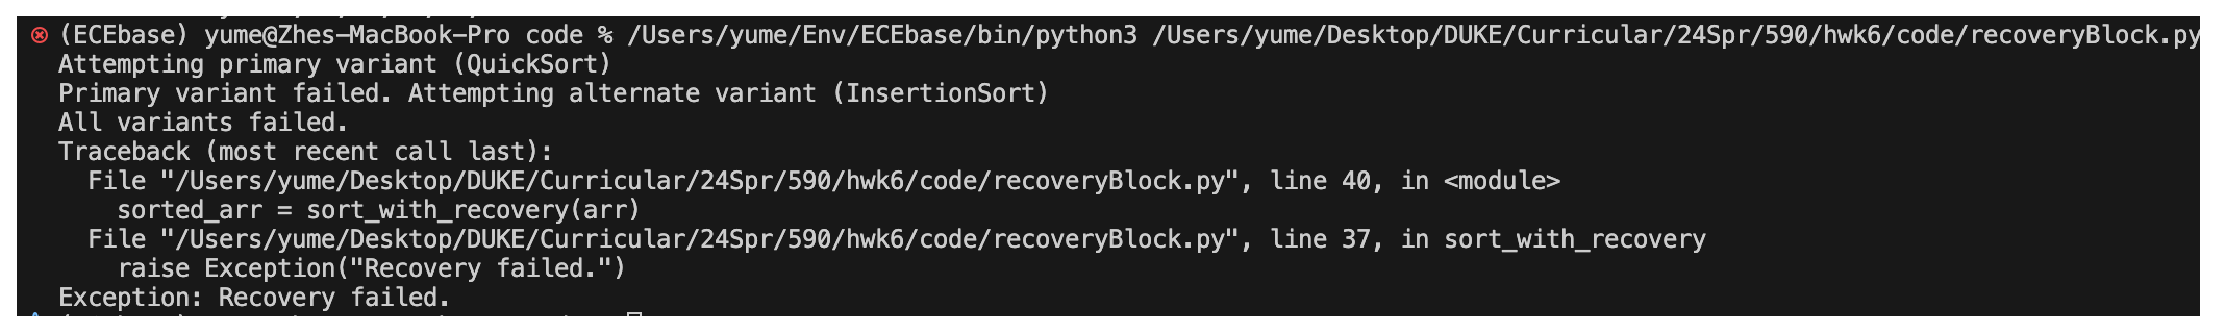
\includegraphics[width=1\textwidth]{image/3.eps}
	\end{center}
	
	
	\section*{Question 3: } 
	\textbf{a.}
	
	No, the program is not fault-free. The reason is that it uses a shared variable counter which is incremented by multiple threads without any form of synchronization mechanism (like mutexes or atomic operations). This leads to a race condition where multiple threads may read, increment, and write back the value of counter concurrently, leading to lost updates. Therefore, not all increments might be successfully reflected in the final value of counter.\\
	\\
	\textbf{b.}
	
	Yes, there is an Atomicity Violation-Related fault (ARB). An atomicity violation occurs when a sequence of operations that should be executed atomically (i.e., as an indivisible operation) is not protected from being interleaved with other operations. In this code, the increment operation (counter = counter + 1;) is expected to happen atomically but is not protected against concurrent access from other threads, leading to an atomicity violation.\\
	\\
	\textbf{c.}
	
	\begin{lstlisting}[language=C]
		#include <pthread.h>
		#include <stdio.h>
		#include <stdlib.h>
		#include <unistd.h>
		
		#define N_THREADS 100
		
		int counter;
		
		void * thread_code(void * arg) {
			counter += 1;
			pthread_exit(0);
		}
		
		void start_threads() {
			int i;
			pthread_t threads[N_THREADS];
			counter = 0;  // Reset counter to 0 before starting threads
			
			for (i = 0; i < N_THREADS; i++) {
				pthread_create(&threads[i], NULL, thread_code, NULL);
			}
			
			for (i = 0; i < N_THREADS; i++) {
				pthread_join(threads[i], NULL);
			}
		}
		
		void test(int nums) {
			int pass = 0;
			for (int i = 0; i < nums; i++) {
				start_threads();
				if (counter == N_THREADS) {
					pass++;
				}
			}
			double passRate = ((double)pass / nums) * 100;
			printf("For %d executions: Passed %d tests. Pass rate: %.2f%%\n", nums, pass, passRate);
		}
		
		int main() {
			int testCounts[] = {10, 100, 1000, 3000, 8000, 10000, 15000};
			int numberOfTests = sizeof(testCounts) / sizeof(testCounts[0]);
			
			for (int i = 0; i < numberOfTests; i++) {
				test(testCounts[i]);
			}
			
			return EXIT_SUCCESS;
		}\end{lstlisting} 
	
	\begin{center}
		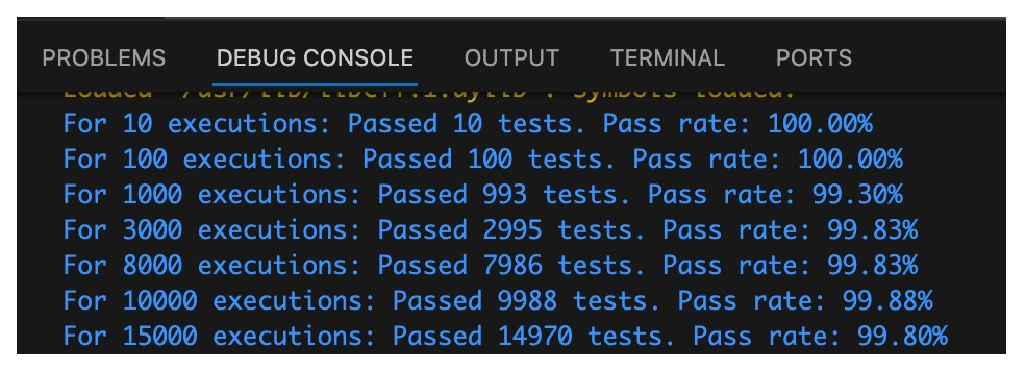
\includegraphics[width=1\textwidth]{image/4.eps}
	\end{center}

	The results indicate a generally high pass rate, with a slight decline as the number of executions increases. As the number of executions grows, the probability of encountering a situation where threads interfere with each other's operations on the shared counter variable increases, leading to occasional failures to achieve the expected final value of the counter.\\
	\\
	\textbf{d.}
	
	Given the context that in a real-world scenario, particularly for applications with potentially billions of queries per second (QPS), even a minor decrease in reliability or a small incidence rate of failure could lead to significant disruptions, the recommendation leans towards returning the program to the development team for further refinement. 
	
	While the pass rates observed are commendably high (ranging from 99.30\% to 99.88\% for varying execution counts), in environments with extremely high QPS, even a 0.12\% failure rate can translate to a substantial number of failures. For instance, at one billion queries, a 0.12\% failure rate would result in 1.2 million failures, potentially affecting a large number of users or transactions.
	
	The existing program, while robust in many respects, may benefit from implementing more sophisticated concurrency control mechanisms. Techniques such as mutexes, semaphores, or atomic operations could enhance the program's ability to manage concurrent access to shared resources more effectively, thereby improving its reliability.
	
	In environments where downtime or errors could have significant financial or reputational repercussions, erring on the side of caution by ensuring the software is as robust as possible is a prudent approach. Returning the program to the development team allows for a thorough review and enhancement of its concurrency handling capabilities, ultimately reducing the risk of failure post-deployment.
	
	In conclusion, considering the critical importance of reliability and fault tolerance in environments with very high QPS, it is advisable to return the program to the development team for further refinement. Enhancing the program's concurrency management capabilities and conducting extensive stress testing under conditions simulating real-world loads will help ensure that it meets the stringent reliability requirements necessary for successful deployment in such demanding scenarios.
\end{document}